\header{
    \section{Ah ! Que nos pères} \label{ah-que-nos-peres}
    %
    
    \insertComment{Chanson datant probablement du moyen âge, retranscrite par Delphin Balleyguier au 19ème siècle, reprenant des couplets datant d'au moins 1741}{}
}

\enluminure{4}{\href{https://www.youtube.com/watch?v=QehZfWdEh14}{A}}{h !} Que nos pères étaient heureux \bissimple
\\Quand ils étaient à table.
\\Le vin coulait à côté d'eux \bissimple
\\Ça leur était fort agréable.
\\\\\textbf{Refrain :}
\\Et ils buvaient à pleins tonneaux
\\Comme des trous
\\Comme des trous, morbleu!
\\Bien autrement que nous, morbleu!
\\Bien autrement que nous.
\\\\Ils n'avaient ni riches buffets \bissimple
\\Ni verres de Venise.
\\Mais ils avaient des gobelets \bissimple
\\Aussi grands que leurs barbes grises.
\\\\Ils ne savaient ni le latin \bissimple
\\Ni la théologie,
\\Mais ils avaient le goût du vin \bissimple,
\\C'était là leur philosophie.
\\\\Quand ils avaient quelque chagrin \bissimple
\\Ou quelque maladie
\\Ils plantaient là le médecin \bissimple
\\Apothicaire et pharmacie.
\\\\Et quand le petit Dieu Amour \bissimple
\\Leur apportait quelques donzelles
\\Sans peur, sans crainte et sans detour \bissimple
\\Ils plantaient là la demoiselle.
\breakpage
\\\\Celui qui planta le Provins %%\bissimple
\\Celui qui planta le bon vin,
\\Au doux pays de France,
\\Dans l'éclat du rubis divin %%\bissimple
\\Dans l'éclat de rubis du vin,
\\Il a planté notre espérance.
\\\\\\\textbf{Refrain final :}
\\Amis buvons à pleins tonneaux
\\Comme des trous
\\Comme des trous, morbleu!
\\L'avenir est à nous, morbleu!
\\L'avenir est à nous.
\\
\begin{figure}[h!]
\centering
   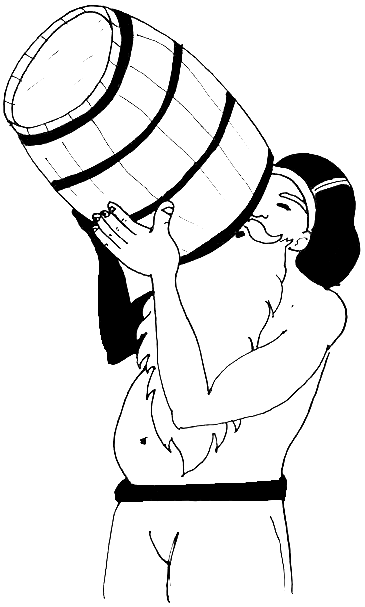
\includegraphics[width=0.6\textwidth]{images/ah_que_nos_peres.png}
 \end{figure}

\breakpage